\documentclass[letterpaper, notitlepage]{revtex4-1}
\usepackage{longtable}
\usepackage{graphicx} 
\usepackage{sidecap}
\usepackage{balance}
\usepackage{amsmath}
\usepackage{amssymb}
\usepackage{amssymb}
\newcommand*{\QEDA}{\hfill\ensuremath{\blacksquare}}%
\newcommand*{\QEDB}{\hfill\ensuremath{\square}}%
\usepackage{siunitx}
\usepackage[none]{hyphenat}
\usepackage[margin=0.7in]{geometry}
\usepackage{esvect}
\usepackage{braket}
\usepackage{listings}
\usepackage{epstopdf}
\usepackage{subfigure}
\usepackage{color} %red, green, blue, yellow, cyan, magenta, black, white
\usepackage{verbatim}
\usepackage{mwe}
\definecolor{mygreen}{RGB}{28,172,0} % color values Red, Green, Blue
\definecolor{mylilas}{RGB}{170,55,241}
\graphicspath{{Figures/}}
\DeclareSIUnit\uvrms{\micro\volt{}_{RMS}}

\begin{document}
\lstset{language=Matlab,%
    %basicstyle=\color{red},
    breaklines=true,%
    morekeywords={matlab2tikz},
    keywordstyle=\color{blue},%
    morekeywords=[2]{1}, keywordstyle=[2]{\color{black}},
    identifierstyle=\color{black},%
    stringstyle=\color{mylilas},
    commentstyle=\color{mygreen},%
    showstringspaces=false,%without this there will be a symbol in the places where there is a space
    numbers=left,%
    numberstyle={\tiny \color{black}},% size of the numbers
    numbersep=9pt, % this defines how far the numbers are from the text
    emph=[1]{for,end,break},emphstyle=[1]\color{red}, %some words to emphasise
    %emph=[2]{word1,word2}, emphstyle=[2]{style},    
}

\title{EE 315\\Project Milestone}
\author{Thomas Flores and Samuel Lenius}
\affiliation{}
\date{\today}
\maketitle

\section{Inverter Chain}
We design an inverter chain to buffer the comparator outputs and drive a load capacitance of \SI{50}{\femto\farad}. Using a FO4 approach, we can write the total necessary number of stages as
\begin{equation}
N=\log_4\left(\frac{C_{load}}{C_{inv}}\right)
\end{equation}
where $C_{inv}$ is the input capacitance for the unit inverter. Our unit inverter is sized using minimum sized nmos transistors such that $W_n=\SI{180}{\nano\metre}$ and $L_n=\SI{90}{\nano\metre}$. To reduce on resistance variation but to also minimize delay, the pmos is sized such that $W_p=2*W_n$ and $L_n=L_p$. To determine the input capacitance for our unit inverter, we set up the test bench as show in Figure \ref{fig:TestBench}.
\begin{figure}[h]
\begin{center}
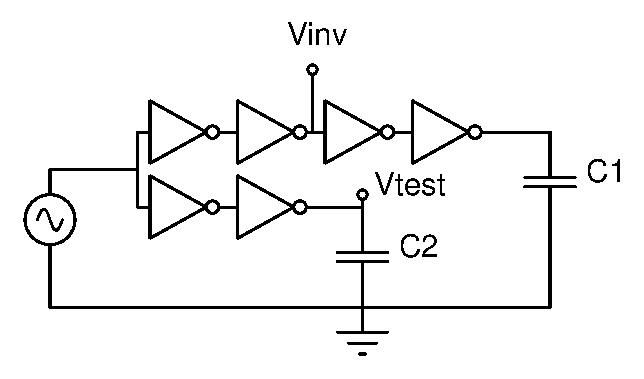
\includegraphics[width=0.4\textwidth]{Inverter_Design/TestBench.eps}
\caption{Test bench for extracting the input capacitance of the unit inverter.}.
\label{fig:TestBench}
\end{center}
\end{figure}
Here, we input a step response into a chain of inverters and probe the output at two points. At $V_{test}$ we probe the output into $C_2$ and sweep $C_2$ from \SI{0.3}{\femto\farad} to \SI{0.6}{\femto\farad}. We extract the rise and fall time from $0.1$ to $0.9\cdot V_{DD}$ and match to the rise and fall time at $V_{inv}$. Using this approach, we find that $C_{inv}=\SI{0.52}{\femto\farad}$. Therefore, our inverter chain with FO4 will have
\begin{equation}
N=\log_4\left(\frac{\SI{50}{\femto\farad}}{\SI{0.52}{\femto\farad}}\right)\approx3
\end{equation}
and is shown below in Figure \ref{fig:InvChain}.
\begin{figure}[h]
\begin{center}
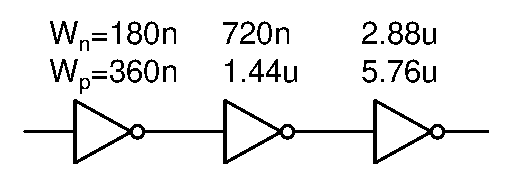
\includegraphics[width=0.3\textwidth]{Inverter_Design/Inverter_Chain.eps}
\caption{Inverter chain design to drive a capacitive load of \SI{50}{\femto\farad}. All lengths are minimum length = \SI{90}{\nano\metre}}.
\label{fig:InvChain}
\end{center}
\end{figure}

\section{DC Analysis}

\section{Regeneration Time Constant}

\section{Sample Rate}

\section{Thermal Noise Voltage}
We can model the circuit using the small signal model. We therefore have a gain of
\begin{equation}
A_v=-\frac{g_{m_n}}{g_{ds_{n}}+g_{ds_{p}}-g_{m_p}}
\end{equation}
The thermal noise sources from the nmos and pmos transistors can be written at the output as
\begin{equation}
\overline{V_{out,tot}^2}=2\cdot\left(\frac{4kT\gamma}{g_{m_p}}+\gamma g_{m_n}\left(r_{o,n}||r_{o,p}\right)\frac{kT}{C_L}\right)
\end{equation}

We can then refer this to the input using the previously derived gain equation to find
\begin{equation}
\overline{V^2_{in,tot}}=\frac{\overline{V_{out,tot}^2}}{\left|A_v\right|^2}\left(\gamma\left(g_{m_n}+g_{m_p}\right)\left(r_{o,n}||r_{o,p}\right)\frac{kT}{C_L}\right)\left(\frac{g_{ds_{n}}+g_{ds_{p}}-g_{m_p}}{g_{m_n}}\right)^2
\end{equation}





\end{document}

